\section*{Exercício 3: Carrinho de Compras}

\begin{figure}[htbp]
    \centering
    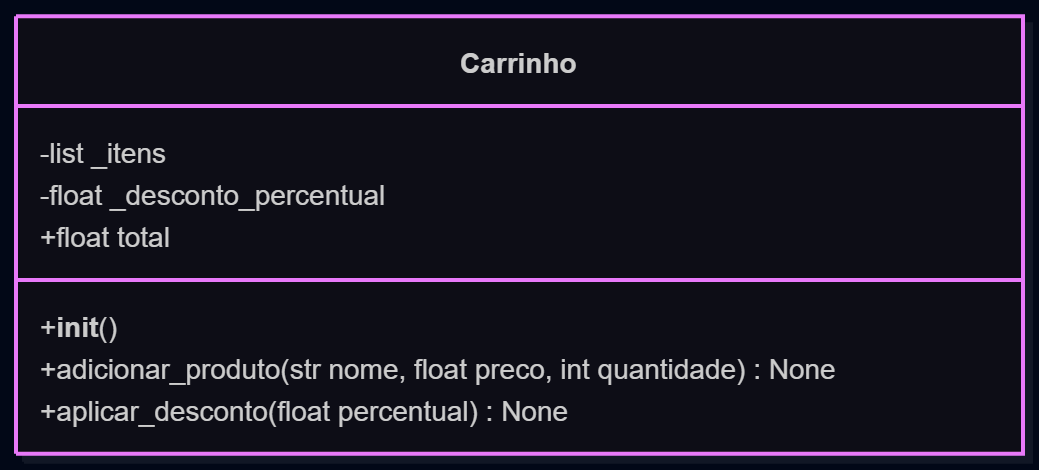
\includegraphics[width=0.65\textwidth]{carrinho_uml.png}
    \caption{Modelagem de classes UML da entidade Carrinho.}
    \label{fig:carrinho_uml_claro}
\end{figure}

\begin{enumerate}
    \item \textbf{Quais funcionalidades foram implementadas?}
    
    Foi desenvolvida a classe \texttt{Carrinho} com suporte completo às seguintes operações de negócio:
    \begin{itemize}
        \item Inicialização do estado interno com uma lista de itens vazia e percentual de desconto zerado.
        \item Adição de itens unitários ou múltiplos informando nome, preço e parâmetro opcional de quantidade (com valor padrão unitário).
        \item Validação defensiva de entrada: rejeição de quantidade menor ou igual a zero com lançamento da exceção \\ \texttt{ValueError("Quantidade inválida")}.
        \item Aplicação de desconto percentual acumulável sobre o valor total do carrinho.
        \item Cálculo dinâmico do montante total via método \texttt{total()}, que percorre os itens acumulando os subtotais e aplicando o abatimento percentual configurado.
    \end{itemize}

    \item \textbf{Quais testes foram criados?}
    
    No módulo \texttt{test\_carrinho.py}, foram implementados 6 casos de teste automatizados com o \textit{Pytest} para validar as regras obrigatórias:
    \begin{itemize}
        \item \texttt{teste\_carrinho\_vazio()}: confirma que uma nova instância do carrinho inicia com total igual a 0.
        \item \texttt{teste\_produto\_100\_total\_100()}: verifica a inserção de um único produto (Mouse de R\$ 100,00) totalizando R\$ 100,00.
        \item \texttt{teste\_dois\_produtos\_total\_250()}: valida a inserção cumulativa de dois produtos distintos (Mouse de R\$ 100,00 e Teclado de R\$ 150,00), totalizando R\$ 250,00.
        \item \texttt{teste\_produtos\_com\_quantidade\_total\_300()}: \\ testa o parâmetro explícito de quantidade (Mouse de R\$ 100,00 com quantidade 3), resultando no total de R\$ 300,00.
        \item \texttt{teste\_total\_500\_10\_porcento\_desconto()}: valida o abatimento percentual de 10\% sobre um carrinho de R\$ 500,00, confirmando o total final de R\$ 450,00.
        \item \texttt{teste\_quantidade\_invalida()}: valida o fluxo de exceção ao tentar inserir um produto com quantidade igual a 0, assegurando o disparo de \texttt{ValueError} via \texttt{pytest.raises}.
    \end{itemize}

    \begin{figure}[htbp]
        \centering
        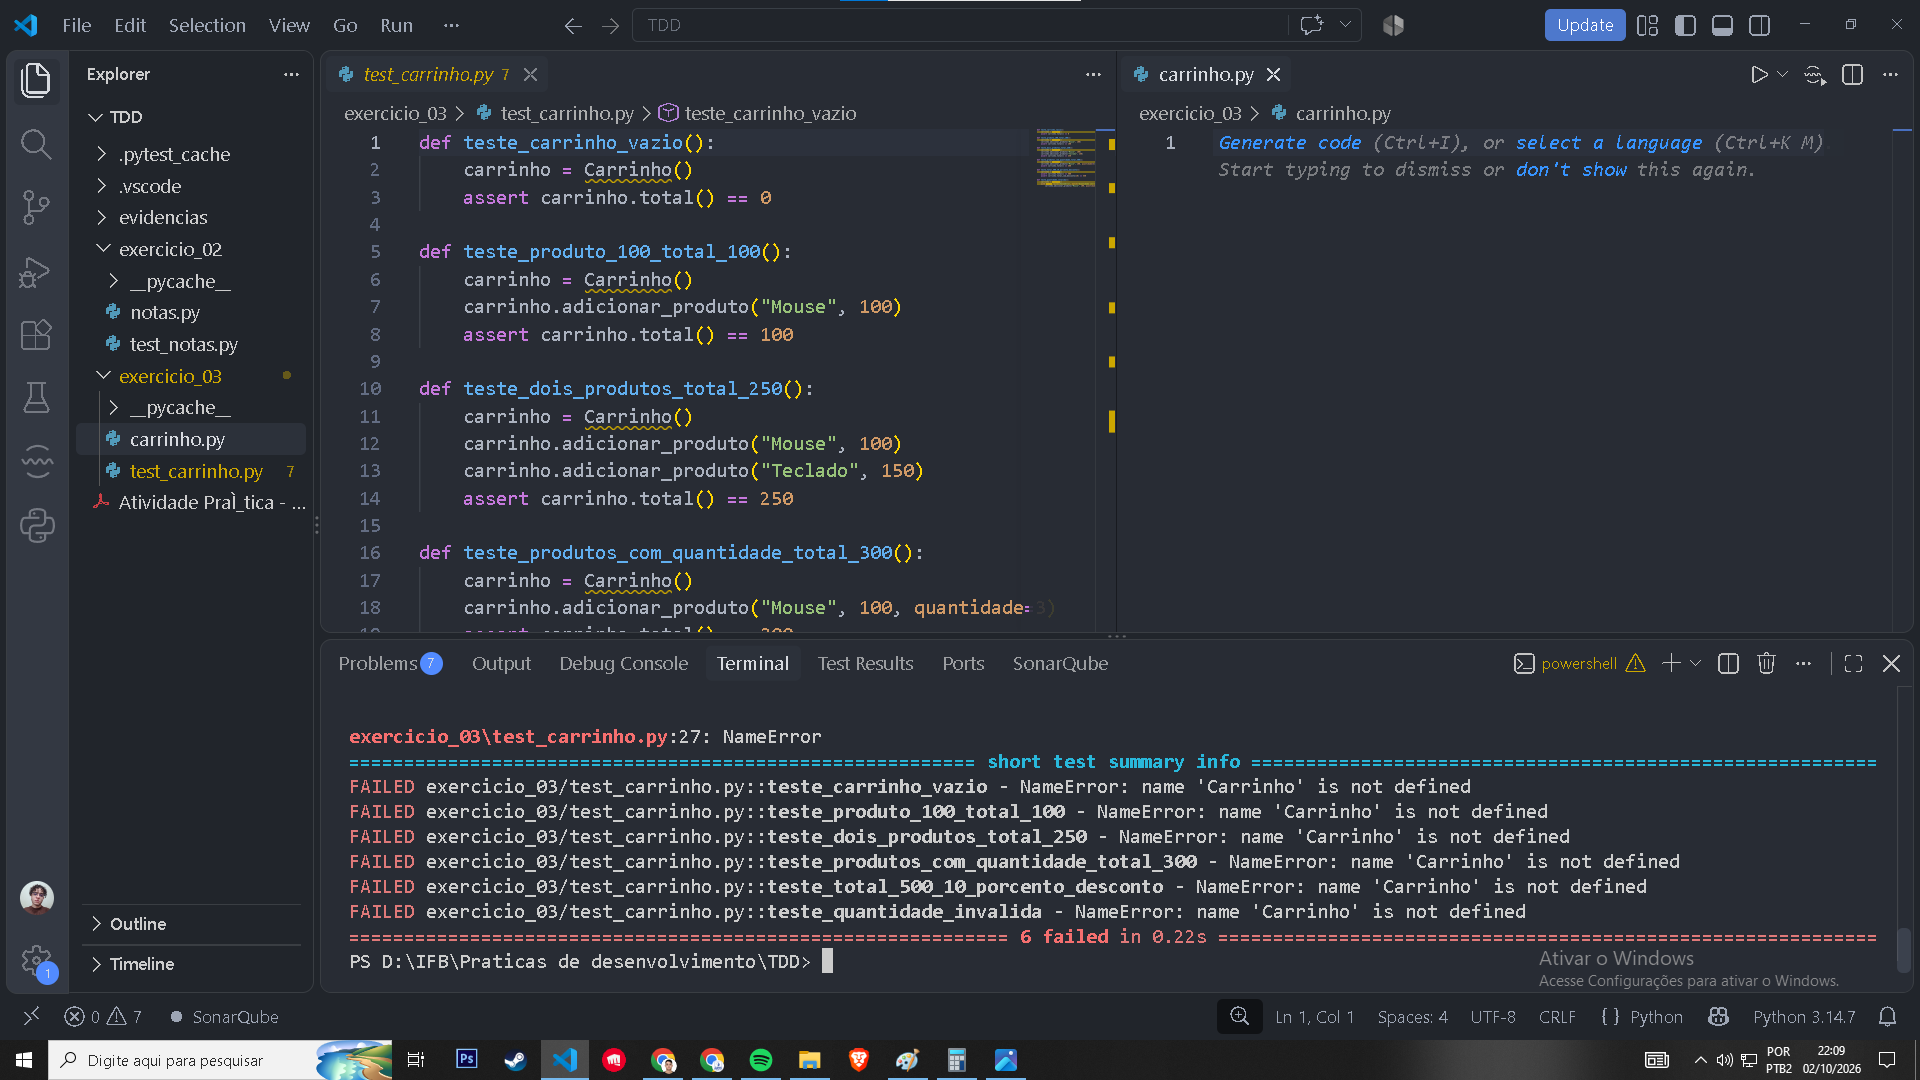
\includegraphics[width=0.92\textwidth]{ex03_red.png}
        \caption{Evidência da fase RED: execução prévia dos testes acusando NameError pela ausência da classe.}
        \label{fig:ex03_red}
    \end{figure}

    \vspace{1.0cm}
    
    \item \textbf{Qual foi a principal dificuldade encontrada durante o desenvolvimento?}
    
    A principal dificuldade foi a utilização do Python para a definição de classe. Questões como a obrigatoriedade da referência explícita \texttt{self} nos métodos de instância, o controle estrito de indentação de blocos e a manipulação de estruturas de dados dinâmicas (dicionários e listas por compreensão no cálculo do somatório) exigiram atenção. Além disso, compreender o ciclo do TDD na modelagem de classes — garantindo que a interface pública dos métodos fosse planejada primeiro a partir do teste unitário antes de qualquer definição da estrutura interna da classe — exigiu uma mudança de raciocínio em relação ao desenvolvimento tradicional.

    \begin{figure}[htbp]
        \centering
        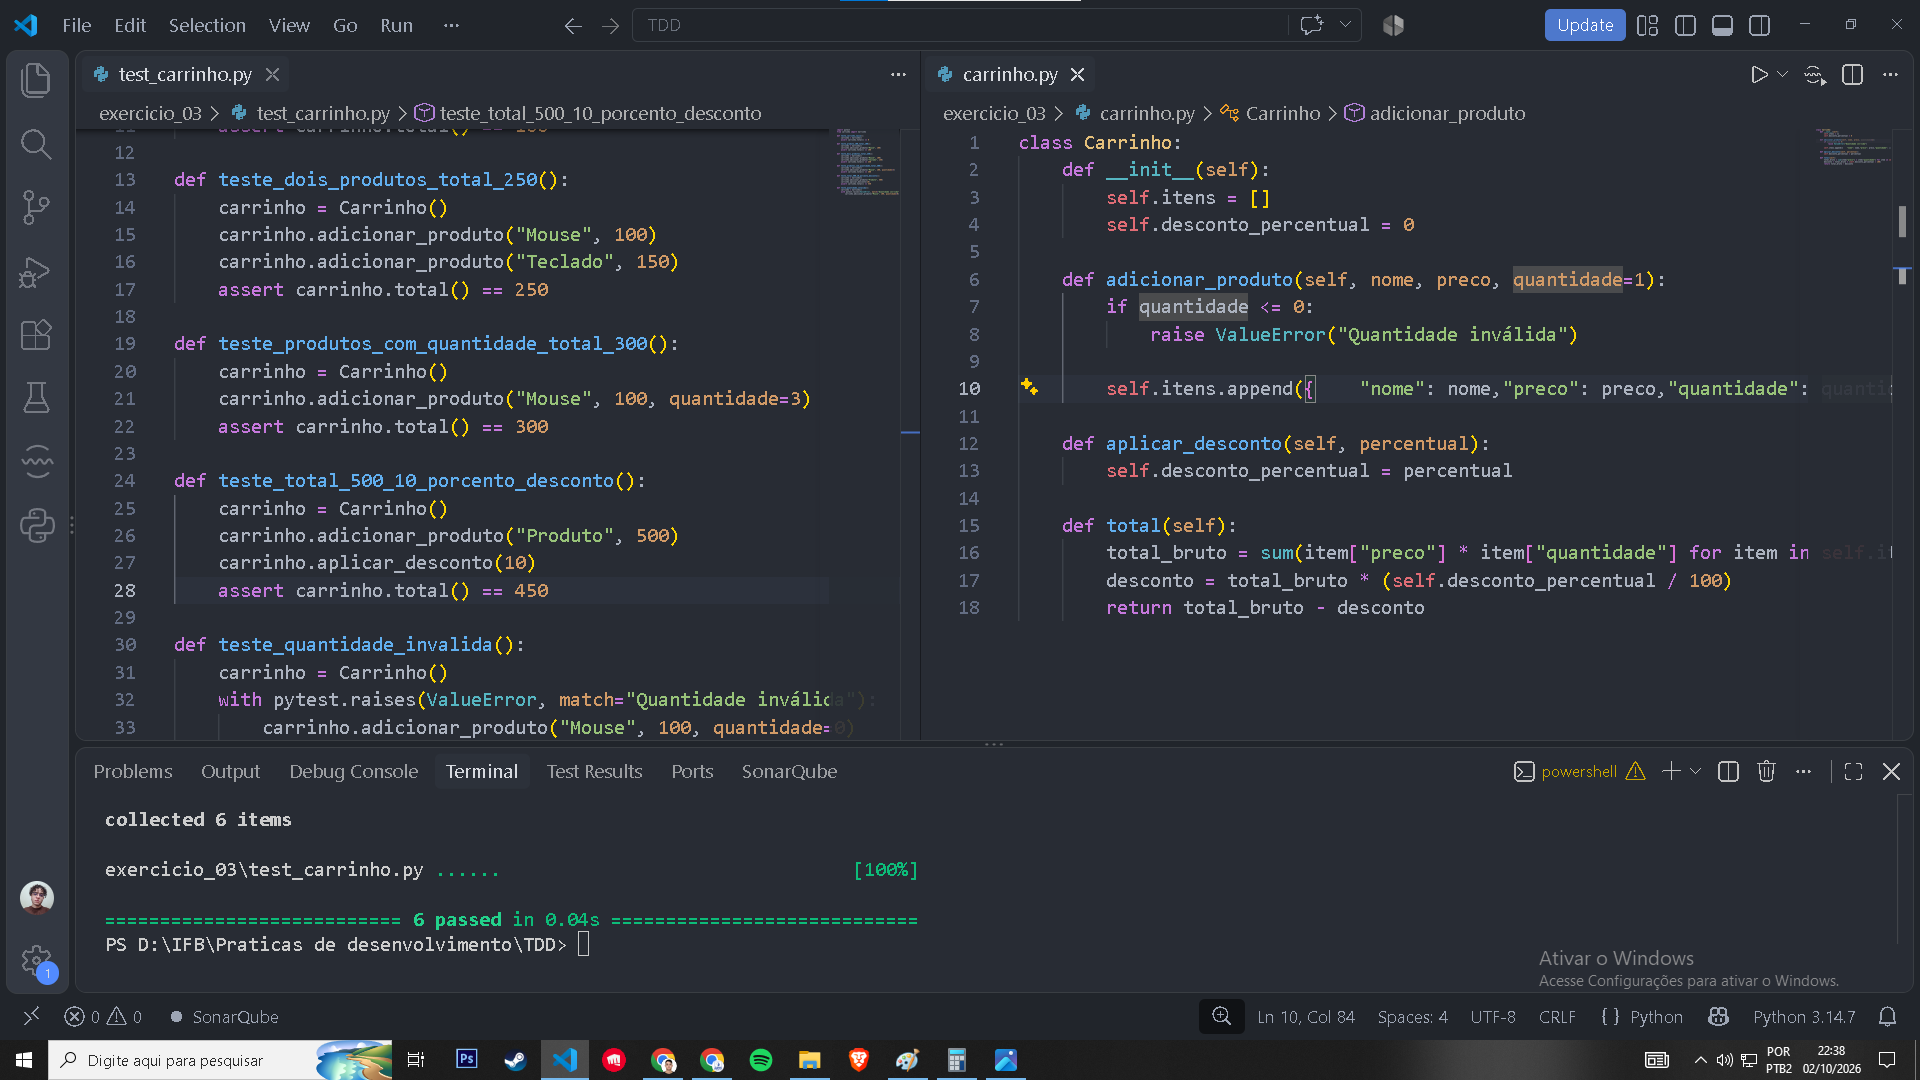
\includegraphics[width=0.92\textwidth]{ex03_green.png}
        \caption{Evidência da fase GREEN: implementação da classe satisfazendo todos os 6 testes no Pytest.}
        \label{fig:ex03_green}
    \end{figure}

    \begin{figure}[htbp]
        \centering
        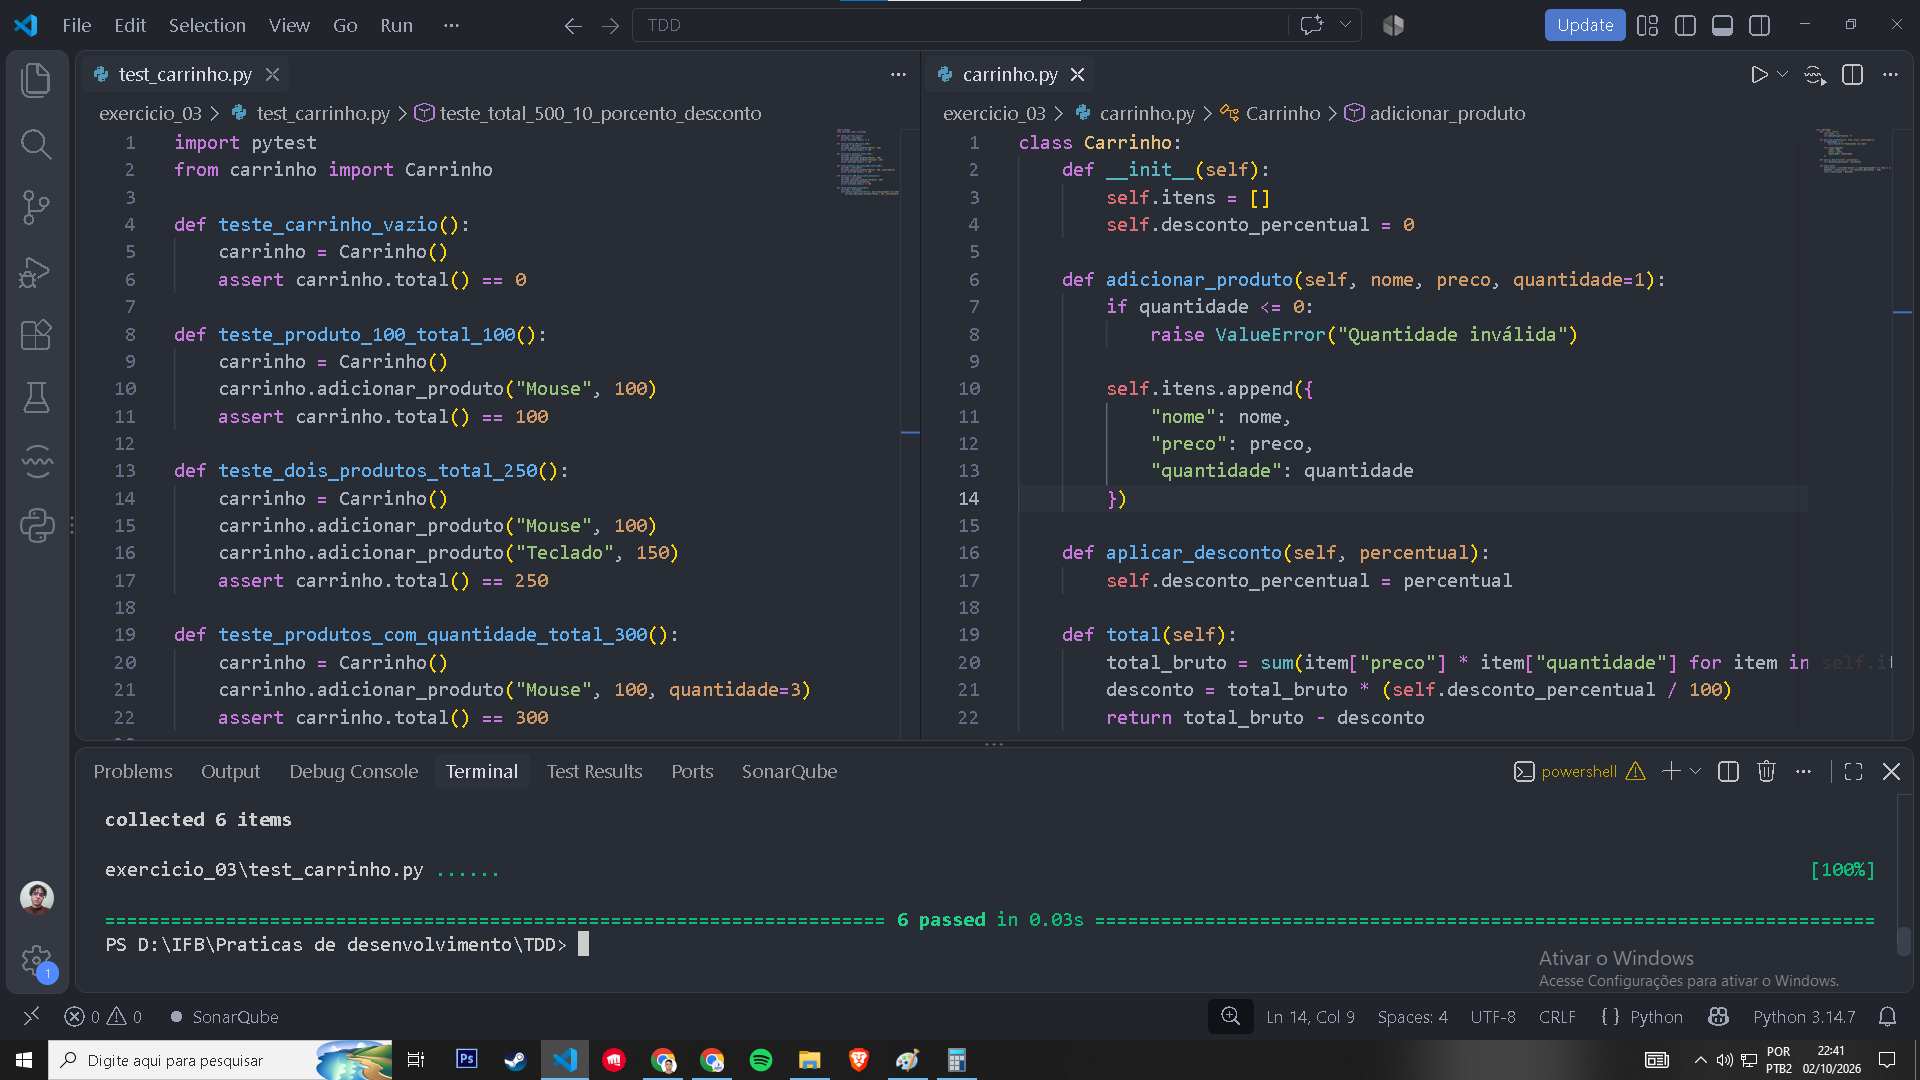
\includegraphics[width=0.92\textwidth]{ex03_refactor.png}
        \caption{Evidência da fase REFACTOR: suíte integral com os 6 testes passando com código consolidado.}
        \label{fig:ex03_refactor}
    \end{figure}
\end{enumerate}